% Copyright (C) 2007 Technical University of Liberec.  All rights reserved.
%
% Please make a following reference to Flow123d on your project site if you use the program for any purpose,
% especially for academic research:
% Flow123d, Research Centre: Advanced Remedial Technologies, Technical University of Liberec, Czech Republic
%
% This program is free software; you can redistribute it and/or modify it under the terms
% of the GNU General Public License version 3 as published by the Free Software Foundation.
%
% This program is distributed in the hope that it will be useful, but WITHOUT ANY WARRANTY;
% without even the implied warranty of MERCHANTABILITY or FITNESS FOR A PARTICULAR PURPOSE.
% See the GNU General Public License for more details.
%
% You should have received a copy of the GNU General Public License along with this program; if not,
% write to the Free Software Foundation, Inc., 59 Temple Place - Suite 330, Boston, MA 021110-1307, USA.
%
%%%%%%%%%%%%%%%%%%%%%%%%%%%%%%%%%%%%%%%%%%%%%%%%%%%%%%%%%%%%%%%%%%
%
% use PDFLatex to compile this
%

\documentclass[a4paper]{article}

%\usepackage{rotating}
%\usepackage{pdflscape}

\usepackage[bbgreekl]{mathbbol}
\usepackage{amssymb, amsmath, amsthm, stmaryrd}
\newtheorem{theorem}{Theorem}

\usepackage{array}
\usepackage{longtable}
\usepackage[usenames,dvipsnames]{color}   %colors
%\usepackage{colortbl}   %colorful tables
\usepackage{tabularx,tikz}
\usepackage{graphicx} %[dvips]
% it is note used \usepackage{cooltooltips}

%these two can be found in caption package
%\usepackage{caption}
%\usepackage{subcaption}

\usepackage[numbers]{natbib}
\usepackage{ulem}
\usepackage{etoolbox}
\usetikzlibrary{arrows,matrix}


%%%%%%%%%%%%%%%%%%%%%%%%%%%%%%%%%%%%%%%%%%%%%%%%%%%%%%%%%%%%%%%%%%%%%%%%%%%%
% macro for units 
% \def\UNIT#1#2{\ifstrempty{#2}{}{%
% \ifstrequal{#2}{1}{\mathrm{#1}}{\mathrm{#1}^{#2}}%
% }}
% \def\units#1#2#3{\ifstrempty{#1#2#3}{$[-]$}{$[ \UNIT{kg}{#1}\UNIT{m}{#2}\UNIT{s}{#3} ]$}}       %with brackets
% \def\unitss#1#2#3{\ifstrempty{#1#2#3}{$-$}{$ \UNIT{kg}{#1}\UNIT{m}{#2}\UNIT{s}{#3} $}}  %without brackets

\newtheorem{lemma}[theorem]{Lemma}

%%%%%%%%%%%%%%%%%%%% specific math macros
\def\abs#1{\lvert#1\rvert}
\def\Abs#1{\bigl\lvert#1\bigr\rvert}
\def\avg#1{\{\!\{#1\}\!\}}
\def\d {\,{\rm d}}
\def\dist{\operatorname{dist}}
\def\div{\operatorname{div}}
\def\dn{\d\nnu}
\def\ep{\vc\varepsilon}
\def\ff{\vc f}
\def\grad{\nabla}
\def\jmp#1{\llbracket #1 \rrbracket}
\def\Lapl{\Delta}
\def\Natural{\mathbf N}
\def\nn{\vc n}
\def\nnu{\vc\nu}
\def\norm#1{\|#1\|}
\def\ol{\overline}
\def\pbar{\overline p}
\def\prtl{\partial}
\def\qq{\vc q}
\def\Real{{\mathbf R}}
\def\tn#1{{\mathbb{#1}}}    % tensor
\def\tr{\operatorname{tr}}
\def\U{\vc U}
\def\ubar{\overline\uu}
\def\ul{\underline}
\def\uu{\vc u}
\def\V{\vc V}
\def\vc#1{\mathbf{\boldsymbol{#1}}}     % vector
\def\vv{\vc v}
\def\weakly{\rightharpoonup}
\def\xx{\vc x}
\def\yy{{\vc y}}

\newcommand{\eq}[1]{\begin{equation}#1\end{equation}}
\newcommand{\ml}[1]{\begin{multline}#1\end{multline}}
\newcommand{\mls}[1]{\begin{multline*}#1\end{multline*}}

\newcommand{\note}[2]{{\color{blue} \textbf{ #1:} \textit{#2}}}
%% ini_table members
%%%%%%%%%%%%%%%%%%%% specific math macros

\newcommand{\opm}{ % plus and minus in circle
  {\mathbin{
    \mathchoice
      {\buildcirclepm{\displaystyle     }{0.14ex}{0.95}{0.05ex}{.7}}
      {\buildcirclepm{\textstyle        }{0.14ex}{0.95}{0.05ex}{.7}}
      {\buildcirclepm{\scriptstyle      }{0.13ex}{0.955}{0.04ex}{.55}}
      {\buildcirclepm{\scriptscriptstyle}{0.08ex}{0.95}{0.03ex}{.45}}
  }} 
}
\newcommand\buildcirclepm[5]{%
  \begin{tikzpicture}[baseline=(X.base), inner sep=-#5, outer sep=-.65]
    \node[draw,circle,line width=#4] (X)  {\footnotesize\raisebox{#2}{\scalebox{#3}{$#1\pm$}}};
  \end{tikzpicture}%
}


%%%%%%%%%%%%%%%%%%%%%%%%%%%%%%%%%%%%%%%%%%%%%%%%%%%%%%%%%%%%%%%%%%%%%%%%%%%%%%%%%%%%%%%%%%%%% BEGIN DOCUMENT
\begin{document}

\title{Mixed-dimensional models of linear elasticity and poroelasticity}
\author{Jan Březina and Jan Stebel}
\maketitle

\section{Introduction}


\begin{figure}[h]
\centering
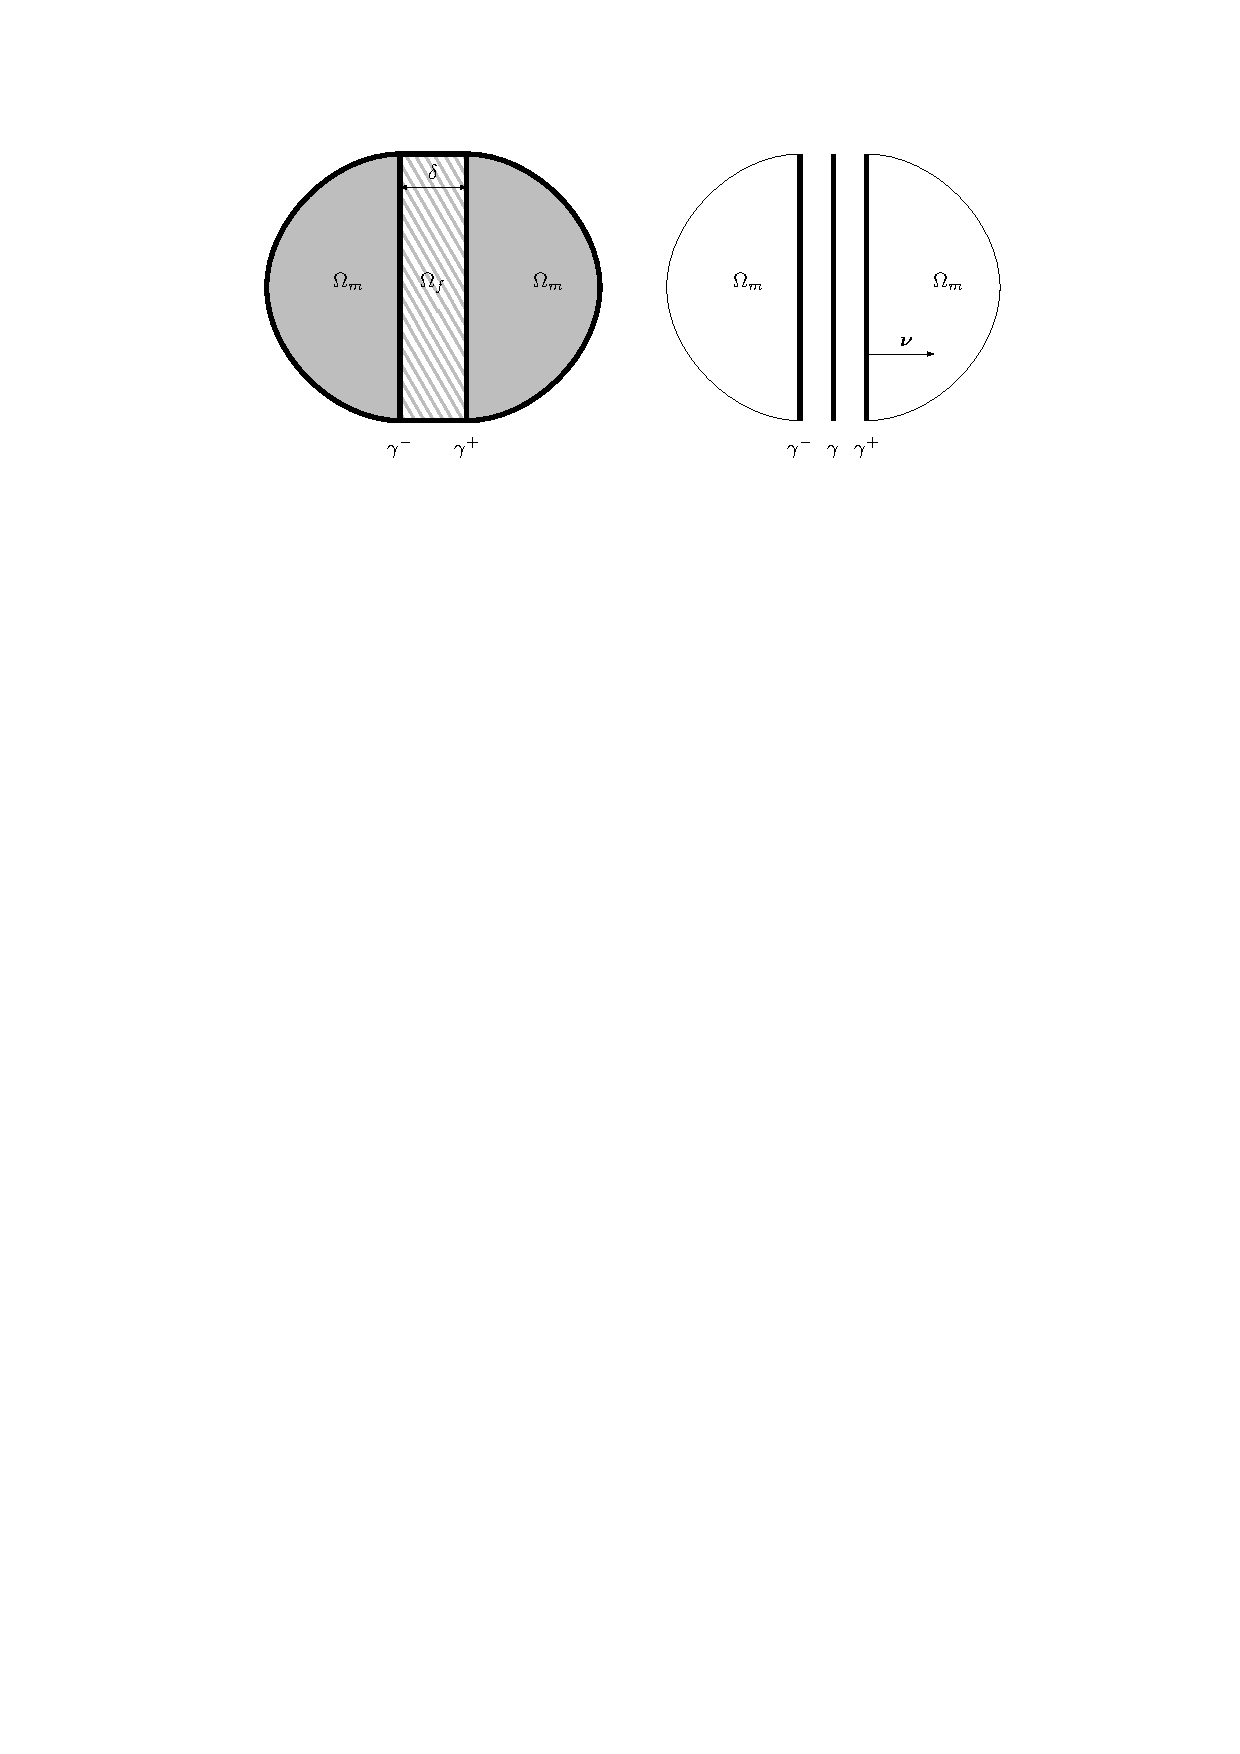
\includegraphics[width=\textwidth]{figures/omegas}
\label{fig:omegas}
\caption{The domain of the full model (left) and the reduced geometry (right).}
\end{figure}

We consider a bounded, simply connected domain $\Omega \subset \Real^d$, $d\in\{2,3\}$ with Lipschitz boundary, which contains a thin layer
\eq{ \Omega_f := \Omega\cap \big((-\tfrac\delta2,\tfrac\delta2)\times\Real^{d-1}\big) }
called fracture, with aperture $\delta>0$ (see Figure \ref{fig:omegas}).
The surrounding domain $\Omega_m:=\Omega\setminus\overline\Omega_f$, so-called matrix, is divided into two parts, which are interacting with $\Omega_f$ via two interfaces
\eq{ \gamma^+:=\Omega\cap\big( \{\tfrac\delta2\}\times \Real^{d-1}\big), \quad \gamma^-:=\Omega\cap\big( \{ -\tfrac\delta2\}\times \Real^{d-1}\big). }
Further, we introduce the reduced fracture
\eq{ \gamma:=\Omega\cap\big(\{0\}\times\Real^{d-1}\big) }
lying in the center of $\Omega_f$.
By $\nnu$ we denote the unit normal vector to $\gamma$ in the direction from $\gamma^-$ to $\gamma^+$.
The symbol $\prtl\Omega$ stands for the boundary of $\Omega$, while $\prtl\gamma$ shall denote the relative boundary of $\gamma$.

We shall derive a model of poroelasticity on the reduced geometry consisting of $\Omega_m$ and $\gamma$.
The starting point is the Biot system:
\begin{subequations}
\label{eq:biot}
\begin{align}
    \label{eq:lin_el}
    -\div \bbsigma + \nabla(\alpha p) &= \ff &&\mbox{ in }\Omega_m\cup\Omega_f,\\
\label{eq:biot_darcy}    \prtl_t\left(Sp + \div(\alpha\uu)\right) + \div\qq &= g &&\mbox{ in }\Omega_m\cup\Omega_f,
\end{align}
\end{subequations}
where $\bbsigma$ is the stress tensor given by the Hooke law
\eq{ \bbsigma = \tn C\nabla\uu, }
$\tn C$ is the $4^{\rm th}$-order elasticity tensor, $\uu$ the displacement, $\alpha$ the Biot effective stress (???), $p$ the pressure, $\ff$ the body force, $S$ the storativity, $g$ the fluid source and $\qq$ the flux given by the Darcy law:
\[ \quad \qq = -\tn K\nabla p \]
via the hydraulic conductivity tensor $\tn K$.
On the interface between $\Omega_m$ and $\Omega_f$ we require that
\eq{ p,\uu,\qq\cdot\nnu,\bbsigma\nnu \mbox{ are continuous on } \gamma^\pm. }

In what follows, we shall assume that the physical parameters $\alpha,S,\tn C,\tn K$ are constant in $\Omega_m$, $\Omega_f$, respectively.
To distinguish values on the interfaces $\gamma^\pm$ we shall use the subscripts ``$m$'' and ``$f$'', i.e. $\alpha_m := \alpha_{|\Omega_m}$, $\alpha_f := \alpha_{|\Omega_f}$ etc.
In addition, it is assumed that $\tn C_*$ and $\tn K_*$, $*\in\{m,f\}$, have the usual symmetries:
\eq{ \forall i,j,k,l=1,\ldots,d:~ [\tn C_*]_{ijkl}=[\tn C_*]_{jikl}=[\tn C_*]_{ijlk}=[\tn C_*]_{klij}, }
\eq{ \tn K_* = \tn K_*^\top, }
and are positive definite:
\eq{ \label{eq:pos_def_C} \forall\tn A\in\Real^{d\times d}_{sym}:~\tn C_*[\tn A]:\tn A \ge C_1|\tn A|^2, }
\eq{ \forall\vv\in\Real^d:~\tn K_*\vv\cdot\vv \ge C_2|\vv|^2,\quad *\in\{m,f\}. }
Here $|\tn A|$ denotes the Frobenius norm, i.e. $|\tn A|^2=\tn A:\tn A$.
A further natural requirement is that $\nnu$ is an eigenvector of $\tn K_f$, i.e.
\eq{\label{eq:normal_conductivity} \tn K_f\nnu = k_f\nnu, }
where $k_f>0$ is the hydraulic conductivity in orthogonal direction to $\gamma$.




\section{Tangential and normal calculus in fracture}

Let $\tn P := \nnu\otimes\nnu$ be the orthogonal projector to $\gamma$.
For any $\vv\in\Real^d$ and $\tn A\in\Real^{d\times d}$ we shall define the orthogonal decomposition into normal and tangential direction to $\gamma$:
\eq{ \vv = \tn P\vv + (\tn I-\tn P)\vv =:\vv_\nu + \vv_\tau, }
\eq{ \tn A = \tn A\tn P + \tn A(\tn I-\tn P) =: \tn A_\nu + \tn A_\tau. }
Likewise we decompose differential operators acting on vector- and tensor-valued functions:
\eq{ \label{eq:grad_sc} \nabla f = (\nabla f)_\nu + (\nabla f)_\tau =: \nabla_\nu f + \nabla_\tau f, }
\eq{ \label{eq:grad_vc} \nabla\vv = (\nabla\vv)_\nu + (\nabla\vv)_\tau =: \nabla_\nu\vv + \nabla_\tau\vv, }
\eq{ \div\vv = \div\vv_\nu + \div\vv_\tau =: \div_\nu\vv + \div_\tau\vv, }
\eq{ \label{eq:div_tn} \div\tn A = \div(\tn P\tn A) + \div((\tn I-\tn P)\tn A) =: \div_\nu\tn A + \div_\tau\tn A. }
Let $w$ be a function defined in $\Omega_f$.
We denote its trace on $\gamma^\pm$ as follows:
\eq{ w^{\opm}(\xx) := w(\xx\pm\tfrac\delta2\nnu), ~\xx\in\gamma, }
and introduce the average and the jump between the traces:
\eq{ \avg{w} := \frac{w^\oplus+w^\ominus}2,\quad \jmp{w} := w^\oplus-w^\ominus. }
When integrating across the fracture, we shall write
\[ \int w\dn := \int w(\cdot+s\nnu)\d s. \]
The symbol $\overline w$ will denote the integral mean of $w$ across the fracture aperture, i.e.
\eq{\label{eq:def_mean} \overline w:=\frac1\delta\int_{-\tfrac\delta2}^{\tfrac\delta2} w \dn. }
Then it holds:
\eq{ \label{eq:int_grad_nu_sc}
\int_{-\tfrac\delta2}^{\tfrac\delta2}\nabla_\nu f\dn = \int_{-\tfrac\delta2}^{\tfrac\delta2}\nnu\frac{\rm d}{{\rm d}s}\left(f(\cdot+s\nnu)\right)\d s = \jmp{f}\nnu,
}
\eq{ \label{eq:div_nu_vc}
\int_{-\tfrac\delta2}^{\tfrac\delta2}\div_\nu\vv\dn = \int_{-\tfrac\delta2}^{\tfrac\delta2}\nnu\cdot\frac{\rm d}{{\rm d}s}\left(\vv(\cdot+s\nnu)\right)\d s = \jmp{\vv}\cdot\nnu,
}
\eq{ \label{eq:int_grad_nu_vc} \int_{-\tfrac\delta2}^{\tfrac\delta2}\nabla_\nu\vv\dn = \jmp{\vv}\otimes\nnu, }
\eq{ \label{eq:int_div_nu_tn} \int_{-\tfrac\delta2}^{\tfrac\delta2}\div_\nu\tn A \dn = \jmp{\tn A^\top}\nnu. }
We also have the Green formula:
\eq{ \int_\gamma(\div_\tau\vv)w = \int_{\prtl\gamma}(\vv\cdot\nn)w - \int_\gamma\vv\cdot\nabla_\tau w, }
where $\nn$ denotes the unit outward normal to $\partial\gamma$.



\section{Continuum-fracture model for elasticity}

Our aim is to obtain an equation for the averages $(\overline\uu,\overline p)$ in $\gamma$.
To do so, we integrate \eqref{eq:lin_el} over the fracture aperture:
\eq{\label{eq:lin_el_int} -\int_{-\tfrac\delta2}^{\tfrac\delta2}\div\bbsigma\dn + \int_{-\tfrac\delta2}^{\tfrac\delta2}\nabla(\alpha p)\dn = \delta\overline\ff. }
Next, we decompose the integrands on the left hand side of \eqref{eq:lin_el_int} into tangential and normal parts and use the formulae \eqref{eq:int_grad_nu_sc}, \eqref{eq:int_div_nu_tn}.
We get:
\eq{\label{eq:decomp_div_sigma}
\int_{-\tfrac\delta2}^{\tfrac\delta2}\div\bbsigma\dn = \int_{-\tfrac\delta2}^{\tfrac\delta2}\left(\div_\tau\bbsigma + \div_\nu\bbsigma\right) \dn
= \delta\div_\tau\tn C_f\overline{\nabla\uu} + \jmp{\bbsigma}\nnu,
}
\eq{\label{eq:decomp_grad_alpha_p} \int_{-\tfrac\delta2}^{\tfrac\delta2}\nabla(\alpha p)\dn = \int_{-\tfrac\delta2}^{\tfrac\delta2} \left(\nabla_\tau(\alpha p) + \nabla_\nu(\alpha p)\right) \dn
= \delta\nabla_\tau(\alpha_f\pbar) + \alpha_f\jmp{p}\nnu.
}
Using \eqref{eq:int_grad_nu_vc} we can express the averaged gradient:
\eq{\label{eq:avg_grad_u} \overline{\nabla\uu} = \nabla_\tau\ubar + \jmp{\uu}\otimes\tfrac{\nnu}\delta. }
Now we turn to approximation of the normal stress $\bbsigma\nnu$ on $\gamma^\pm$.
We define the approximate normal gradient in the positive/negative half of the fracture:
\eq{ \tn G_\nu^\opm = \tn G_\nu^\opm[\uu^\opm,\ubar] := \frac{\pm(\uu^\opm-\ubar)}{\tfrac\delta2}\otimes\nnu = \pm\frac2\delta(\uu^\opm-\ubar)\otimes\nnu. }
Assuming that $\nabla^2\uu$ is bounded in $\Omega_f$, we have that
\eq{ (\nabla_\nu\uu)^\opm = \tn G_\nu^\opm + O(\delta). }
For the tangential gradient we shall use the approximation
\eq{ (\nabla_\tau\uu)^\opm = \nabla_\tau\ubar + O(\delta). }
We can observe that the approximate normal and tangential gradient satisfy
\eq{ \overline{\nabla\uu} = \nabla_\tau\ubar + \avg{\tn G_\nu}. }
Then the approximate normal stress is given by
\eq{\label{eq:def_T} \vc T^\opm = \vc T^\opm[\uu^\opm,\ubar] := \left(\tn C_f\left(\nabla_\tau\ubar + \tn G_\nu^\opm\right)\right)\nnu, }
so that $\bbsigma^\opm\nnu = \vc T^\opm + O(\delta)$.
Collecting \eqref{eq:lin_el_int}, \eqref{eq:decomp_div_sigma}, \eqref{eq:decomp_grad_alpha_p}, \eqref{eq:avg_grad_u} and \eqref{eq:def_T} and neglecting $O(\delta)$ we obtain the averaged counterpart of \eqref{eq:lin_el}:
\eq{ \delta\left(-\div_\tau\tn C_f\left(\nabla_\tau\ubar+\avg{\tn G_\nu}\right) + \nabla_\tau(\alpha_f\pbar)\right) - \jmp{\vc T} + \alpha_f\jmp{p}\nnu = \delta\overline\ff. }
The continuity of $\bbsigma\nnu$ on $\gamma^\pm$ is approximated by the condition
\eq{ (\tn C_m\nabla\uu_{|\Omega_m})\nnu = \vc T^\opm \mbox{ on }\gamma^\pm. }









\section{Continuum-fracture model for flow}

Let us integrate \eqref{eq:biot_darcy} over the fracture aperture.
We get:
\eq{ \label{eq:darcy_int} \prtl_t\left(\delta S\pbar + \int_{-\tfrac\delta2}^{\tfrac\delta2}\div(\alpha\uu)\dn\right) + \int_{-\tfrac\delta2}^{\tfrac\delta2}\div\qq\dn = \delta\overline g. }
The first integral in \eqref{eq:darcy_int} will be rewritten using \eqref{eq:int_div_nu_tn} and \eqref{eq:div_nu_vc}:
\ml{ \label{eq:div_alpha_u_int} \int_{-\tfrac\delta2}^{\tfrac\delta2}\div(\alpha\uu)\dn = \int_{-\tfrac\delta2}^{\tfrac\delta2}\left(\div_\tau(\alpha_f\uu_f) + \div_\nu(\alpha\uu)\right)\dn\\
= \delta\div_\tau(\alpha_f\ubar) + \alpha_f\jmp{\uu}\cdot\nnu. }
Similarly we get
\eq{ \label{eq:div_q_int} \int_{-\tfrac\delta2}^{\tfrac\delta2}\div\qq = \int_{-\tfrac\delta2}^{\tfrac\delta2}\left(\div_\tau\qq + \div_\nu\qq\right) 
= \delta\div_\tau(\tn K_f\overline{\nabla p}) + \jmp\qq\cdot\nnu, }
where
\eq{ \overline{\nabla p} = \nabla_\tau\pbar + \tfrac1\delta\jmp{p}\nnu. }
From the definition of $\div_\tau$ and \eqref{eq:normal_conductivity} it then follows that
\eq{ \label{eq:div_tau_K_gp} \div_\tau(\tn K_f\overline{\nabla p}) = \div_\tau(\tn K_f\nabla_\tau\pbar). }
For the approximation of the normal flux $\qq\cdot\nnu$ on $\gamma^\pm$ we use the approximation
\eq{ \label{eq:approx_p} (\nabla_\nu p)^\opm \approx \frac{\pm(p^\opm-\pbar)}{\tfrac\delta2}\nnu + O(\delta), }
provided that $\nabla^2 p$ is bounded in $\Omega_f$.
Then the approximate normal flux is given by
\eq{ \label{eq:def_F} F^\opm = F^\opm[p^\opm,\pbar] := \pm k_f\frac2\delta(p^\opm-\pbar), }
so that
\eq{ \label{eq:approx_flux} -\qq^\opm\cdot\nnu = \tn K_f\nabla p^\opm\cdot\nnu = k_f(\nabla_\nu p)^\opm\cdot\nnu = F^\opm + O(\delta). }
Now from \eqref{eq:darcy_int}, \eqref{eq:div_alpha_u_int}, \eqref{eq:div_q_int}, \eqref{eq:div_tau_K_gp}, \eqref{eq:def_F} and \eqref{eq:approx_flux} we obtain:
\eq{ \delta\prtl_t\left(S_f\pbar + \div_\tau(\alpha_f\ubar)\right) -\delta\div_\tau(\tn K_f\nabla_\tau\pbar) +\alpha_f\jmp{\prtl_t\uu}\cdot\nnu - \jmp F = \delta\overline g. }
Continuity of flux through $\gamma^\pm$ is approximated by the condition
\eq{ \tn K_m\nabla p_{|\Omega_m}\cdot\nnu = F^\opm \mbox{ on }\gamma^\pm. }




\section{Well-posedness of mixed-dimensional linear elasticity}

In this section we consider only the mechanical part of the problem.
We want to find the displacement fields $\uu:\Omega_m\to\Real^d$ and $\U:\gamma\to\Real^d$ satisfying the following boundary-value problem:
\begin{subequations}\label{eq:lin_el_problem}
\begin{align}
-\div(\tn C_m\nabla\uu) &= \ff &&\mbox{in }\Omega_m,\\
-\delta\div_\tau\left(\tn C_f\left(\nabla_\tau\U+\avg{\tn G_\nu}\right) \right) - \jmp{\vc T} &= \delta\overline\ff &&\mbox{in }\gamma,\\
(\tn C_m\nabla\uu)\nnu &= \vc T^\opm &&\mbox{on }\gamma^\pm,\\
\uu &=\vc0&&\mbox{on }\prtl\Omega_m,\\
\U &=\vc 0&&\mbox{on }\prtl\gamma.
\end{align}
\end{subequations}
Here and in what follows, $\tn G_\nu:=\tn G_\nu[\uu^\opm,\U]$ and $\vc T^\opm=\vc T^\opm[\uu^\opm,\U]$.
Let us define the space 
\eq{ V:=H^1_0(\Omega_m;\Real^d)\times H^1_0(\gamma;\Real^d) }
equipped by the norm $\norm{(\vv,\vc V)}_V := (\norm{\nabla\vv}_{L^2(\Omega)}^2 + \norm{\nabla_\tau\vc V}_{L^2(\gamma)}^2)^{1/2}$ and the forms
\ml{ a((\uu,\U), (\vv,\vc V)) := \int_{\Omega_m}\tn C_m\nabla\uu:\nabla\vv
 + \delta\int_\gamma\tn C_f(\nabla_\tau\U+\avg{\tn G_\nu}):\nabla_\tau\vc V\\
 + \int_\gamma\left(\jmp{\vc T\cdot\vv} - \jmp{\vc T}\cdot\vc V\right), }
\eq{ l((\vv,\vc V)) := \int_{\Omega_m}\ff\cdot\vv + \delta\int_\gamma\overline\ff\cdot\vc V. }
Then the weak formulation of \eqref{eq:lin_el_problem} reads:
\eq{ \label{eq:el_weak} \left.\begin{minipage}{0.7\textwidth}
Find $(\uu,\U)\in V$ such that
\[ \forall(\vv,\vc V)\in V:~a((\uu,\U),(\vv,\vc V)) = l((\vv,\vc V)). \]
\end{minipage}\right\} }
Before establishing the well-posedness of \eqref{eq:el_weak} we prove a suitable Korn type inequality.
\begin{lemma}
There exists a constant $C_3>0$ such that for all $(\vv,\V)\in V$ it holds:
\eq{\label{eq:korn_frac} \norm{\ep\vv}_{L^2(\Omega_m)}^2 + \avg{\norm{\ep_\tau\V+\tfrac12(\tn G_\nu[\vv,\V]+\tn G_\nu^\top[\vv,\V])}_{L^2(\gamma)}^2} \ge C_3\norm{(\vv,\V)}_V^2. }
\end{lemma}
\begin{proof}
Let us assume for contradiction that there is a sequence $\{(\vv_n,\V_n)\}_{n=1}^\infty$ in $V$ such that
\eq{\label{eq:korn_asm_contra} \norm{\ep\vv_n}_{L^2(\Omega_m)}^2 + \avg{\norm{\ep_\tau\V_n+\tfrac12(\tn G_\nu[\vv_n,\V_n]+\tn G_\nu^\top[\vv_n,\V_n])}_{L^2(\gamma)}^2} < \frac1n\norm{(\vv_n,\V_n)}_V^2. }
Without loss of generality we may assume that $\norm{(\vv_n,\V_n)}_V=1$, so that
\eq{\label{eq:korn_weak_vV} (\vv_n,\V_n)\weakly (\vv,\V) \mbox{ weakly in }V, }
where $(\vv,\V)\in V$, passing eventually to a subsequence.
From \eqref{eq:korn_asm_contra} and the Korn inequality in $H^1_0(\Omega_m;\Real^d)$ it follows that
\eq{\label{eq:korn_strong_v} \vv_n\to\vc 0 \mbox{ strongly in }H^1_0(\Omega_m;\Real^d). }
From \eqref{eq:korn_asm_contra} it also follows that
\eq{\label{eq:korn_conv_approx_grad} \ep_\tau\V_n+\tfrac12(\tn G_\nu^\opm[\vv_n^\opm,\V_n]+\tn G_\nu^{\opm\top}[\vv_n^\opm,\V_n]) \to 0 \mbox{ strongly in }L^2(\gamma;\Real^{d\times d}). }
Using this together with \eqref{eq:korn_weak_vV}, \eqref{eq:korn_strong_v} and the definition of $\tn G_\nu^\opm$ we obtain:
\eq{ \ep_\tau\V = \pm\frac1\delta(\V\otimes\nnu+\nnu\otimes\V), }
from which it follows that $\V=\vc 0$.
With help of \eqref{eq:korn_conv_approx_grad} and the compact embeddings $H^1(\Omega_m)\hookrightarrow L^2(\gamma)$ and $H^1(\gamma)\hookrightarrow L^2(\gamma)$ we find that
\eq{ \ep_\tau\V_n\to 0 \mbox{ strongly in }L^2(\gamma;\Real^{d\times d}). }
The Korn inequality in $H^1_0(\gamma)$ then implies
\eq{ \V_n\to\vc 0 \mbox{ strongly in }H^1_0(\gamma;\Real^d). }
Finally, having shown the strong convergence of $\{(\vv_n,\V_n)\}$, we observe that
\eq{ 1 = \norm{(\vv_n,\V_n)}_V \to \norm{(\vv,\V)}_V = 0, }
which is a contradiction.
Therefore the proof is finished.
\end{proof}
In the following lemma we prove the ellipticity of $a$.
\begin{lemma}
The bilinear form $a$ is elliptic in the following sense:
\ml{ \label{eq:a_ellip} \forall(\uu,\U)\in V:~ a((\uu,\U),(\uu,\U))\\
\ge C_1\left(\norm{\nabla\uu}_{L^2(\Omega_m)}^2 + \frac\delta2\norm{\nabla_\tau\U}_{L^2(\gamma)}^2 + \frac2\delta\avg{\norm{\uu-\U}_{L^2(\gamma)}^2}\right), }
where $C_1$ is the constant from \eqref{eq:pos_def_C}.
\end{lemma}
\begin{proof}
For any $(\uu,\U)\in V$ we have:
\ml{\label{eq:a_uu}
a((\uu,\U),(\uu,\U)) = \int_{\Omega_m}\tn C\nabla\uu:\nabla\uu
+ \delta\int_\gamma\avg{\tn C_f(\nabla_\tau\U+\tn G_\nu):\nabla_\tau\U}\\
+ \int_\gamma\jmp{\vc T\cdot(\uu-\U)}.
}
From the definition of $\vc T^\opm$ and $\tn G_\nu^\opm$ we get:
\eq{ \vc T^\opm\cdot(\uu^\opm-\U) = \tn C_f(\nabla_\tau\U+\tn G_\nu^\opm):(\uu^\opm-\U)\otimes\nnu = \pm\frac\delta2\tn C_f(\nabla_\tau\U+\tn G_\nu^\opm):\tn G_\nu^\opm, }
which together with \eqref{eq:a_uu} and \eqref{eq:pos_def_C} yields:
\ml{ \label{eq:a_uu2}
a((\uu,\U),(\uu,\U)) = \int_{\Omega_m}\tn C_m\nabla\uu:\nabla\uu
+ \delta\int_\gamma\avg{\tn C_f(\nabla_\tau\U+\tn G_\nu):(\nabla_\tau\U+\tn G_\nu)}\\
\ge C_1\norm{\ep\uu}_{L^2(\Omega_m)}^2 + \frac\delta2C_1\avg{\norm{\ep_\tau\U+\tfrac12(\tn G_\nu+\tn G_\nu^\top)}_{L^2(\gamma)}^2}.
}
To conclude, we observe that $\nabla_\tau\U:\tn G_\nu^\opm=0$ and $|\tn G_\nu^\opm|=\frac2\delta|\uu^\opm-\U|$.
Hence
\eq{ \norm{\nabla_\tau\U+\tn G_\nu^\opm}_{L^2(\gamma)}^2 = \norm{\nabla_\tau\U}_{L^2(\gamma)}^2 + \frac4{\delta^2}\norm{\uu^\opm-\U}_{L^2(\gamma)}^2. }
Using this in \eqref{eq:a_uu2} we obtain \eqref{eq:a_ellip}.
\end{proof}

It is not difficult to show that $a$ and $l$ are bounded in $V$ provided that $\ff\in L^2(\Omega;\Real^d)$.
Hence we have the following result.

\begin{theorem}
Let $\ff\in L^2(\Omega;\Real^d)$. Then problem \eqref{eq:el_weak} has a unique solution.
\end{theorem}



\subsection{Finite element approximation}






% \section{Mixed formulation for incompressible elastic material}
% TOHLE JE ZATIM JEN PRO ROVINNE PUKLINY
% 
% In this section we shall assume that the elasticity tensor has the form
% \[ c_{ijkl} = \mu(\delta_{ik}\delta_{jl} + \delta_{il}\delta_{jk}) + \lambda\delta_{ij}\delta_{kl}, ~i,j,k,l=1,...,d, \]
% and hence
% \[ \vc\sigma[\uu,p] = 2\mu\ep[\uu] + (\lambda\div\uu - \alpha p)\tn I. \]
% Further we shall assume that the material parameter $\alpha$ is constant in $\Omega_{mi}$, $i=1,2$ and in $\gamma$.
% We aim to derive a formulation which is suitable for the incompressible case, i.e. when $\lambda\to\infty$.
% For this reason we introduce a new quantity
% \[ \phi:=\alpha p-\lambda\div\uu, \]
% so that the stress tensor becomes
% \[ \vc\sigma=\vc\sigma[\uu,\phi] = 2\mu\ep[\uu] - \phi\tn I. \]
% The Biot system in the matrix domain now reads:
% \[ \left.\begin{aligned}
% -\div(2\mu\ep[\uu_i]) + \nabla\phi_i &= \ff\\
% \prtl_t\left(\left(\frac1M+\frac{\alpha^2}\lambda\right)p_i - \frac\alpha\lambda\phi_i\right)-\div(\tn K\nabla p_i) &= g\\
% \div\uu_i - \frac\alpha\lambda p_i + \frac1\lambda\phi_i &= 0
% \end{aligned}\right\} \mbox{ in }\Omega_{mi}, ~i=1,2. \]
% After integrating across the fracture we obtain:
% % The continuum-fracture system for poroelasticity now reads:
% \[ \left.\begin{aligned}
% -\div_\tau(2\delta\mu\ep_\tau[\uu_f]) + \nabla_\tau(\delta\phi_f) + \sum_{i=1}^2\tilde{\vc Q}_i + \tilde{\vc R} &= \delta\overline\ff\\
% \prtl_t\left(\delta\left(\frac1M+\frac{\alpha^2}\lambda\right) p_f - \delta\frac\alpha\lambda\phi_f\right)-\div_\tau(\delta\tn K\nabla_\tau p_f)  + \sum_{i=1}^2F_i &= \delta \overline g\\
% \div_\tau(\delta\uu_f) + \sum_{i=1}^2(\uu_f-\uu_i)\cdot\nn_i - \delta\frac\alpha\lambda p_f + \frac\delta\lambda\phi_f &= 0
% \end{aligned} \right\} \mbox{ in }\gamma, \]
% with the interface conditions
% \[ \left.\begin{aligned}
% \vc\sigma[\uu_i,\phi_i]\nn_i &= \tilde{\vc Q}_i \\
% \tn K\nabla p_i\nn_i &= F_i \end{aligned} \right\} \mbox{ on }\gamma_i,~i=1,2, \]
% where
% \[ \begin{aligned}
% \tilde{\vc Q}_i &= 2\mu\ep_\tau[\uu_f]\nn_i + \frac4\delta\mu(\uu_f-\uu_i) - \phi_f\nn_i, \\
% \tilde{\vc R} &= \sum_{i=1}^2\div_\tau(\mu(\uu_i\otimes\nn_i+\nn_i\otimes\uu_i)). \end{aligned} \]
% One can notice that in the limit $\lambda\to\infty$, the flow and elasticity become independent.



\bibliographystyle{abbrvnat}
\bibliography{flow123d_doc.bib}
%%%%%%%%%%%%%%%%%%%%%%%%%%%%%%%%%%%%%%%%%%%%%%%%%%%%%%%%%%%%%%%%%%%%%%%%%%%%%%%%%%%%%%%%%%%%%%%%%%%%%%%%%%%%%%%%%


\end{document}


